% Created 2014-06-06 Fri 17:52
\documentclass[bigger]{beamer}
\usepackage[utf8]{inputenc}
\usepackage[T1]{fontenc}
\usepackage{fixltx2e}
\usepackage{graphicx}
\usepackage{longtable}
\usepackage{float}
\usepackage{wrapfig}
\usepackage{soul}
\usepackage{textcomp}
\usepackage{marvosym}
\usepackage{wasysym}
\usepackage{latexsym}
\usepackage{amssymb}
\usepackage{hyperref}
\tolerance=1000
\mode<beamer>{\usetheme[compress]{Berlin}}
\usepackage{multirow}
\setbeamertemplate{footline}
  {%
    \begin{beamercolorbox}[colsep=1.5pt]{upper separation line foot}
    \end{beamercolorbox}
    \begin{beamercolorbox}[ht=2.5ex,dp=1.125ex,%
      leftskip=.3cm,rightskip=.3cm plus1fil]{author in head/foot}%
      \leavevmode{\usebeamerfont{author in head/foot}\insertshortauthor}%
      \hfill%
      {\usebeamerfont{institute in head/foot}\usebeamercolor[fg]{institute in head/foot}\insertshortinstitute}%
    \end{beamercolorbox}%
    \begin{beamercolorbox}[ht=2.5ex,dp=1.125ex,%
      leftskip=.3cm,rightskip=.3cm plus1fil]{title in head/foot}%
      {\usebeamerfont{title in head/foot}\insertshorttitle}%
      \hfill%
      {\usebeamerfont{frame number}\usebeamercolor[fg]{frame number}\insertframenumber~/~\inserttotalframenumber}
    \end{beamercolorbox}%
    \begin{beamercolorbox}[colsep=1.5pt]{lower separation line foot}
    \end{beamercolorbox}
  }
\makeatother


%----------------------------------------------------------------------
% Define useful commands
%----------------------------------------------------------------------

\newcommand{\eejj}{\ensuremath{eejj} }
\newcommand{\enujj}{\ensuremath{e\nu jj} }
\newcommand{\mumujj}{\ensuremath{\mu\mu jj} }
\newcommand{\munujj}{\ensuremath{\mu\nu jj} }
\newcommand{\emujj}{\ensuremath{e\mu jj} }
\newcommand{\zjets}{\ensuremath{\text{Z}^{0}}+jets }
\newcommand{\wjets}{\ensuremath{\text{W}^{\pm}}+jets }
\newcommand{\ttbar}{\ensuremath{t\bar{t}} }

\newcommand{\pt}{\ensuremath{p_{\text{T}}} }
\newcommand{\ST}{\ensuremath{S_{\text{T}}} }
\newcommand{\mee}{\ensuremath{m_{\text{ee}}} }
\newcommand{\mll}{\ensuremath{m_{\ell\ell}} }
\newcommand{\mej}{\ensuremath{m_{\text{ej}}} }
\newcommand{\mejmin}{\ensuremath{m_{\text{ej}}^{\text{min}}} }
\newcommand{\mejavg}{\ensuremath{m_{\text{ej}}^{\text{avg}}} }
% \newcommand{\mt}{\ensuremath{m_{\text{T, e}\nu}}}
\newcommand{\mtjnu}{\ensuremath{m_{\text{T, j}\nu}} }


\newcommand{\met}{\ensuremath{\not\!\!{E_{\text{T}}}} }
\newcommand{\mt}{\ensuremath{m_{\text{T, e}\nu}} }

%----------------------------------------------------------------------
% Define useful numbers
%----------------------------------------------------------------------

% Lumi info
\newcommand{\intLumi}{$19.6 \text{ fb}^{-1}$}

% MC scale factors
\newcommand{\enujjWJetsMonteCarloScaleFactor}{0.85 \pm 0.01 \text{ (stat)} \pm 0.01    \text{ (syst)}}
\newcommand{\enujjTTBarMonteCarloScaleFactor}{0.97 \pm 0.02 \text{ (stat)} \pm 0.01    \text{ (syst)}}
% \newcommand{\eejjZJetsMonteCarloScaleFactor} {0.97 \pm 0.01 \text{ (stat)} \pm 0.00004 \text{ (syst)}}
\newcommand{\eejjZJetsMonteCarloScaleFactor} {0.97 \pm 0.01 \text{ (stat)}}

\newcommand{\enujjWJetsMonteCarloScaleFactorMETRescaled}{0.95 \pm 0.02 \text{ (stat)} \pm 0.01 \text{ (syst)}}
\newcommand{\enujjTTBarMonteCarloScaleFactorMETRescaled}{1.07 \pm 0.03 \text{ (stat)} \pm 0.01 \text{ (syst)}}

\newcommand{\enujjWJetsMonteCarloScaleFactorMETandMTRescaled}{0.97 \pm 0.02 \text{ (stat)} \pm 0.01 \text{ (syst)}}
\newcommand{\enujjTTBarMonteCarloScaleFactorMETandMTRescaled}{1.08 \pm 0.03 \text{ (stat)} \pm 0.01 \text{ (syst)}}

\newcommand{\eejjZControlRegionContamination}{4\%}

% Electron scale factors
\newcommand{\electronRecoDataMCScaleFactor}{0.98}
\newcommand{\electronRecoDataMCScaleFactorRelUnc}{1.5}
\newcommand{\electronRecoDataMCScaleFactorSqr}{0.96}

% GEN-level cross-sections (not yet rescaled) 
\newcommand{\wjetsXSection}{37509.0 pb}
\newcommand{\zjetsXSection}{3503.71 pb}
\newcommand{\ttbarXSection}{234 pb}
\newcommand{\stopSChannelXSection}{5.55 pb}
\newcommand{\stopTChannelXSection}{87.1 pb}
\newcommand{\stopTWChannelXSection}{22.2 pb}
\newcommand{\wwXSection}{57.1 pb} % THESE NEED TO BE UPDATED!!!
\newcommand{\wzXSection}{32.3 pb} % THESE NEED TO BE UPDATED!!!
\newcommand{\zzXSection}{8.26 pb} % THESE NEED TO BE UPDATED!!!

% QCD contributions at limit of the analysis
\newcommand{\percentQCDatEEJJLimit}{1\%}
\newcommand{\percentQCDatENuJJLimit}{3\%}

% Closure test contamination
\newcommand{\percentContaminationClosureTest}{5\%}
\newcommand{\percentContaminationClosureTestFinal}{55\%}

% Closure test (low-ST) results
\newcommand{\closureTestLowSTPredicted}{13100}
\newcommand{\closureTestLowSTPredictedUnc}{400}
\newcommand{\closureTestLowSTObserved}{12100}
\newcommand{\closureTestLowSTObservedUnc}{400}
\newcommand{\closureTestLowSTRatio}{1.08}
\newcommand{\closureTestLowSTRatioUnc}{0.05}

% Closure test (mid-ST) results
\newcommand{\closureTestMidSTPredicted}{877}
\newcommand{\closureTestMidSTPredictedUnc}{46.7}
\newcommand{\closureTestMidSTObserved}{600}
\newcommand{\closureTestMidSTObservedUnc}{53}
\newcommand{\closureTestMidSTRatio}{1.46}
\newcommand{\closureTestMidSTRatioUnc}{0.15}

% QCD systematic uncertainty
\newcommand{\qcdSystematicUncertaintyPerEle}{30\%}
\newcommand{\qcdSystematicUncertaintyTwoEle}{60\%}

% TTbar (e-mu-jj) contamination
\newcommand{\emujjContamination}{2\%}
\newcommand{\emujjRecoScaleFactor}{0.974  \pm 0.011 \text{ (stat)}}

% mumujj/munujj scale factors for data-driven background
\newcommand{\mumujjRecoScaleFactor}{97.5 \pm 0.4 \text{ (stat)}}
\newcommand{\munujjRecoScaleFactor}{97.2 \pm 0.5 \text{ (stat)}}

% Shape uncertainties
\newcommand{\enujjWJetsShapeUncertainty}{5.92\%}
\newcommand{\enujjTTBarShapeUncertainty}{8.17\%}
\newcommand{\eejjZJetsShapeUncertainty}{8.70\%}

% EES uncertainties
\newcommand{\electronEnergyScaleUncBarrel}{0.4\%}
\newcommand{\electronEnergyScaleUncEndcap}{4.1\%}

% EER uncertainties
\newcommand{\electronEnergyResolutionUncBarrel}{1.006}
\newcommand{\electronEnergyResolutionUncEndcap}{1.015}

% lumi uncertainty
\newcommand{\lumiUncertainty}{2.6\%}

% limits
\newcommand{\eejjObservedLimit}{1005}
\newcommand{\eejjExpectedLimit}{1030}
\newcommand{\enujjObservedLimit}{845}
\newcommand{\enujjExpectedLimit}{890}

\newcommand{\enujjObservedLimitCombined}{845}
\newcommand{\enujjExpectedLimitCombined}{932}

\newcommand{\eejjObservedLimitNoSyst}{1010}
\newcommand{\eejjExpectedLimitNoSyst}{1030}
\newcommand{\enujjObservedLimitNoSyst}{850}
\newcommand{\enujjExpectedLimitNoSyst}{895}

\newcommand{\eejjObservedLimitMuon}{1015}
\newcommand{\eejjExpectedLimitMuon}{980}
\newcommand{\enujjObservedLimitMuon}{825}
\newcommand{\enujjExpectedLimitMuon}{890}


\newcommand{\lowBetaExpectedLimit}{790}
\newcommand{\lowBetaObservedLimit}{635}

\makeatletter
\newcommand\ChangeItemFont[3]{%
\renewcommand{\itemize}[1][]{%
  \beamer@ifempty{##1}{}{\def\beamer@defaultospec{#1}}%
  \ifnum \@itemdepth >2\relax\@toodeep\else
    \advance\@itemdepth\@ne
    \beamer@computepref\@itemdepth% sets \beameritemnestingprefix
    \usebeamerfont{itemize/enumerate \beameritemnestingprefix body}%
    \usebeamercolor[fg]{itemize/enumerate \beameritemnestingprefix body}%
    \usebeamertemplate{itemize/enumerate \beameritemnestingprefix body begin}%
    \list
      {\usebeamertemplate{itemize \beameritemnestingprefix item}}
      {\def\makelabel####1{%
          {%
            \hss\llap{{%
                \usebeamerfont*{itemize \beameritemnestingprefix item}%
                \usebeamercolor[fg]{itemize \beameritemnestingprefix item}####1}}%
          }%
        }%
  \ifnum\@itemdepth=1\relax
    #1%
  \else
  \ifnum\@itemdepth=2\relax
    #2%
  \else
  \ifnum\@itemdepth=3\relax
    #3%
  \fi%
  \fi%
  \fi%
  }
  \fi%
  \beamer@cramped%
  \raggedright%
  \beamer@firstlineitemizeunskip%
}}
\makeatother

\mode<beamer>{\usecolortheme{bear}}
\mode<beamer>{\titlegraphic{\includegraphics[width=0.2\textwidth]{brown-logo}}}
\providecommand{\alert}[1]{\textbf{#1}}

\title{PDF Uncertainties for LQ1 (EXO-12-041)}
\author{Edmund Berry}
\date{Tuesday, June 3, 2014}
\hypersetup{
  pdfkeywords={},
  pdfsubject={},
  pdfcreator={Emacs Org-mode version 7.8.11}}

\author[Edmund Berry]{\alert{Edmund Berry}}
\begin{document}

\maketitle


\section{Introduction}
\label{sec-1}
\subsection{Introduction}
\label{sec-1-1}
\begin{frame}
\frametitle{Introduction}
\label{sec-1-1-1}
\begin{itemize}

\item Slides show how to find PDF uncertainty on LQ signal
\label{sec-1-1-1-1}%

\item Method follows from LQ3 analysis:
\label{sec-1-1-1-2}%
\begin{itemize}

\item \href{http://cms.cern.ch/iCMS/jsp/analysis/admin/analysismanagement.jsp?ancode=EXO-12-030}{\alert{EXO-12-030}}
\label{sec-1-1-1-2-1}%
\end{itemize} % ends low level

\item LQ3 analysis method taken from prescription on arXiv:
\label{sec-1-1-1-3}%
\begin{itemize}

\item \href{http://arxiv.org/abs/hep-ph/0605240}{\alert{arXiv:hep-ph/0605240}}
\label{sec-1-1-1-3-1}%

\item \href{http://arxiv.org/abs/1101.0538}{\alert{arXiv:1101.0538}}
\label{sec-1-1-1-3-2}%
\end{itemize} % ends low level
\end{itemize} % ends low level
\end{frame}
\section{Procedure}
\label{sec-2}
\subsection{Variables}
\label{sec-2-1}
\begin{frame}
\frametitle{Variables stored in ntuples}
\label{sec-2-1-1}
\begin{itemize}

\item Three vectors:
\label{sec-2-1-1-1}%
\begin{itemize}

\item \texttt{PDFCTEQWeights} (53 elements per event, \texttt{CTEQ})
\label{sec-2-1-1-1-1}%

\item \texttt{PDFMSTWWeights} (41 elements per event, \texttt{MSTW})
\label{sec-2-1-1-1-2}%

\item \texttt{PDFNNPDFWeights} (101 elements per event, \texttt{NNPDF})
\label{sec-2-1-1-1-3}%
\end{itemize} % ends low level

\item First element of vector: mean weight (\texttt{mean})
\label{sec-2-1-1-2}%

\item Other elements of vector: varied weight (\texttt{varied})
\label{sec-2-1-1-3}%
\begin{itemize}

\item Each represents a weight from varying a parameter
\label{sec-2-1-1-3-1}%
\end{itemize} % ends low level

\item For each vector element, $i \neq 0$ of each PDF:
\label{sec-2-1-1-4}%
\begin{itemize}

\item PDF weight = \texttt{varied} / \texttt{mean}
\label{sec-2-1-1-4-1}%
\end{itemize} % ends low level
\end{itemize} % ends low level
\end{frame}
\begin{frame}
\frametitle{Variables to be defined}
\label{sec-2-1-2}
\begin{itemize}

\item for LQ of mass $m$, define four N(event) quantities:
\label{sec-2-1-2-1}%
\begin{itemize}

\item $U_m^0$: N(\alert{unweighted} MC events) in sample initially
\label{sec-2-1-2-1-1}%

\item $U_m^f$: N(\alert{unweighted} MC events) passing final selection
\label{sec-2-1-2-1-2}%

\item $W_m^0$: N(\alert{PDF weighted} MC events) in sample initially
\label{sec-2-1-2-1-3}%

\item $W_m^f$: N(\alert{PDF weighted} MC events) passing final selection
\label{sec-2-1-2-1-4}%
\end{itemize} % ends low level

\item Now define acceptance for LQ of mass $m$:
\label{sec-2-1-2-2}%
\begin{itemize}

\item $AU_m = \frac{U_m^f}{U_m^0}$
\label{sec-2-1-2-2-1}%

\item $AW_m = \frac{W_m^f}{W_m^0}$
\label{sec-2-1-2-2-2}%
\end{itemize} % ends low level

\item We are interested in the \% change in acceptance:
\label{sec-2-1-2-3}%
\begin{itemize}

\item $\Delta A = 100 \cdot \left[\left(\frac{AW_m}{AU_m} \right) - 1\right] = 100 \cdot \left[\left(\frac{W_m^f}{W_m^0} \cdot \frac{U_m^0}{U_m^f} \right) - 1\right]$
\label{sec-2-1-2-3-1}%
\end{itemize} % ends low level
\end{itemize} % ends low level
\end{frame}
\subsection{Plots}
\label{sec-2-2}
\begin{frame}
\frametitle{Example values of $\Delta A$ for M(LQ) = 300, eejj}
\label{sec-2-2-1}
%% Plot
\label{sec-2-2-1-1}

\centering
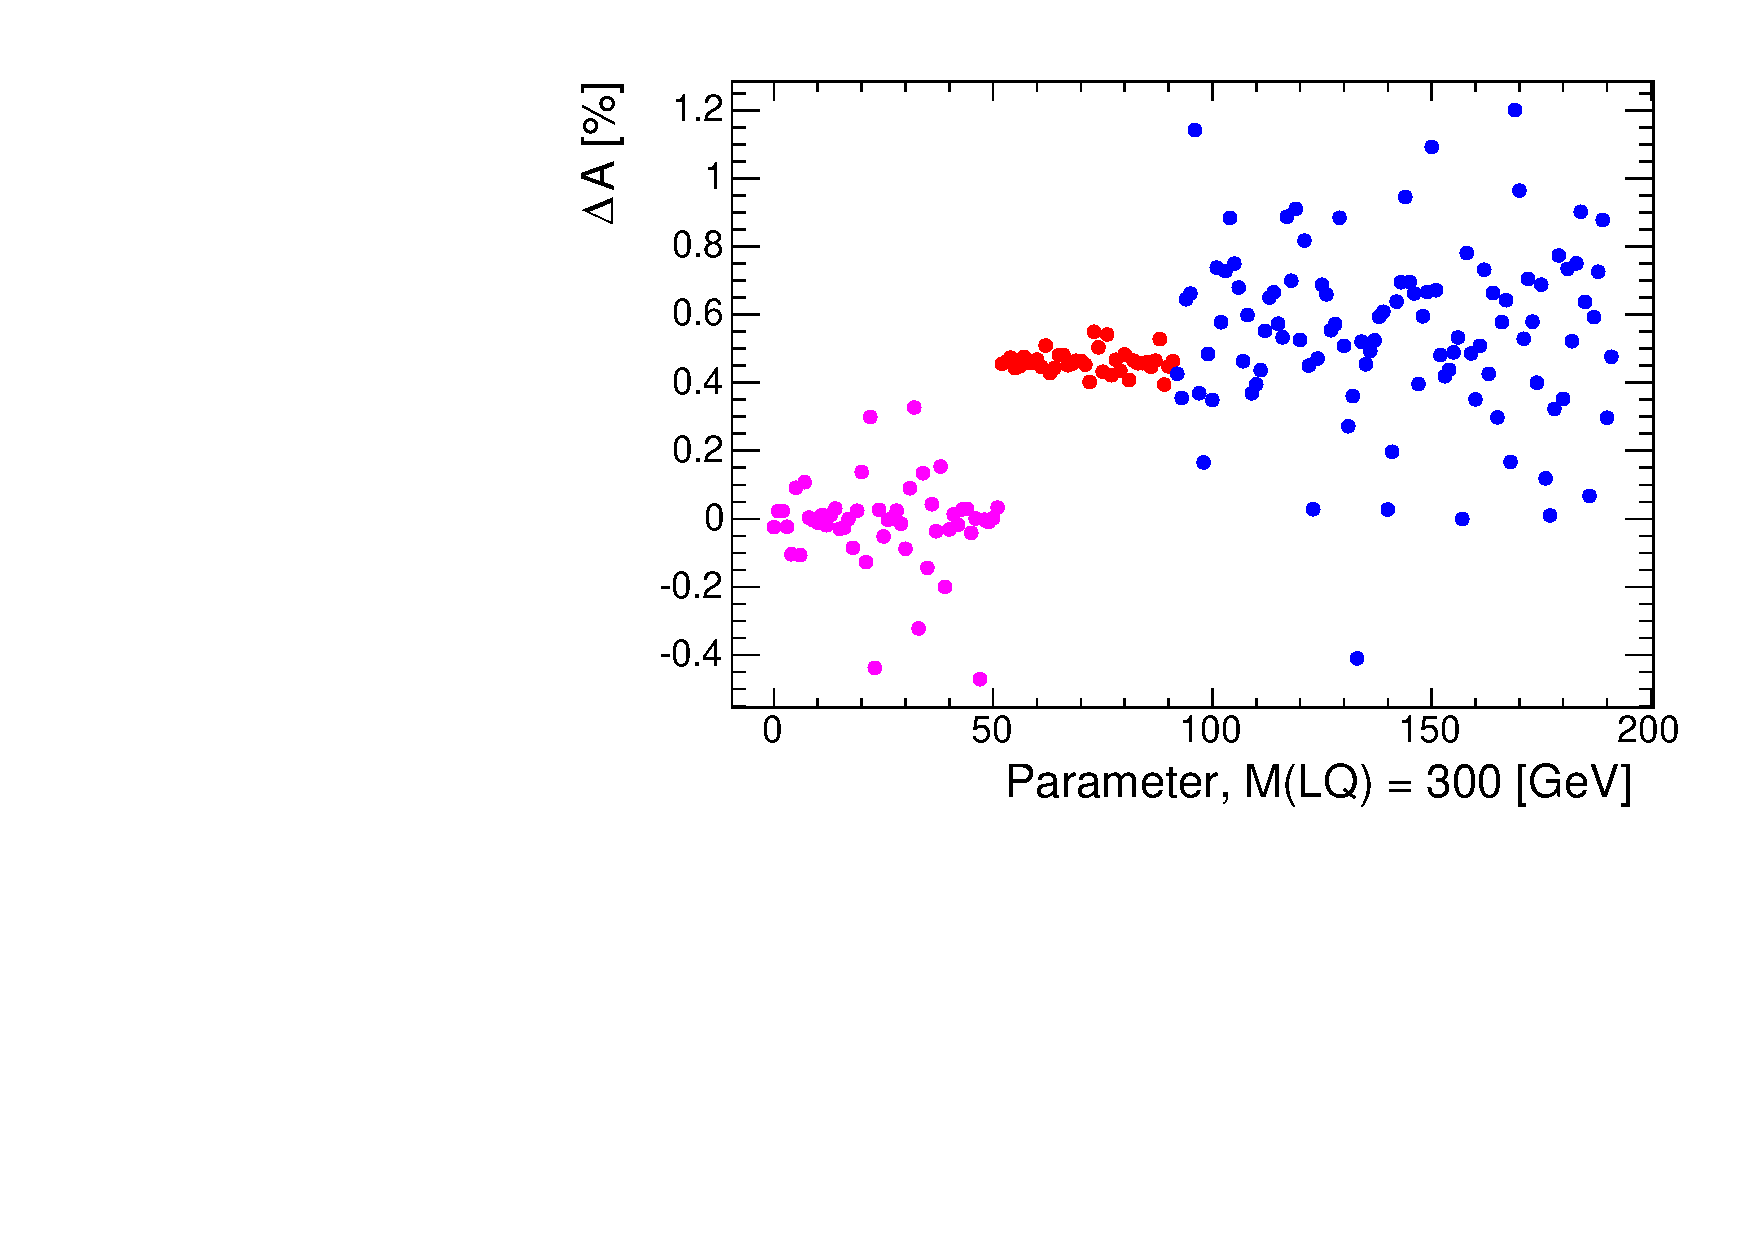
\includegraphics[width=0.6\textwidth]{fig/eejj_300_2D.pdf}
%% Text
\label{sec-2-2-1-2}

\centering
\begin{itemize}

\item Pink: \texttt{CTEQ}, Red: \texttt{MSTW}, Blue: \texttt{NNPDF}
\label{sec-2-2-1-2-1}%

\item $x$-axis: PDF parameter number
\label{sec-2-2-1-2-2}%

\item $y$-axis: $\Delta A$ (defined last slide)
\label{sec-2-2-1-2-3}%
\end{itemize} % ends low level
\end{frame}
\section{Results}
\label{sec-3}
\subsection{Results}
\label{sec-3-1}
\begin{frame}
\frametitle{PDF uncertainty: eejj signal}
\label{sec-3-1-1}
%% Plot
\label{sec-3-1-1-1}

\centering
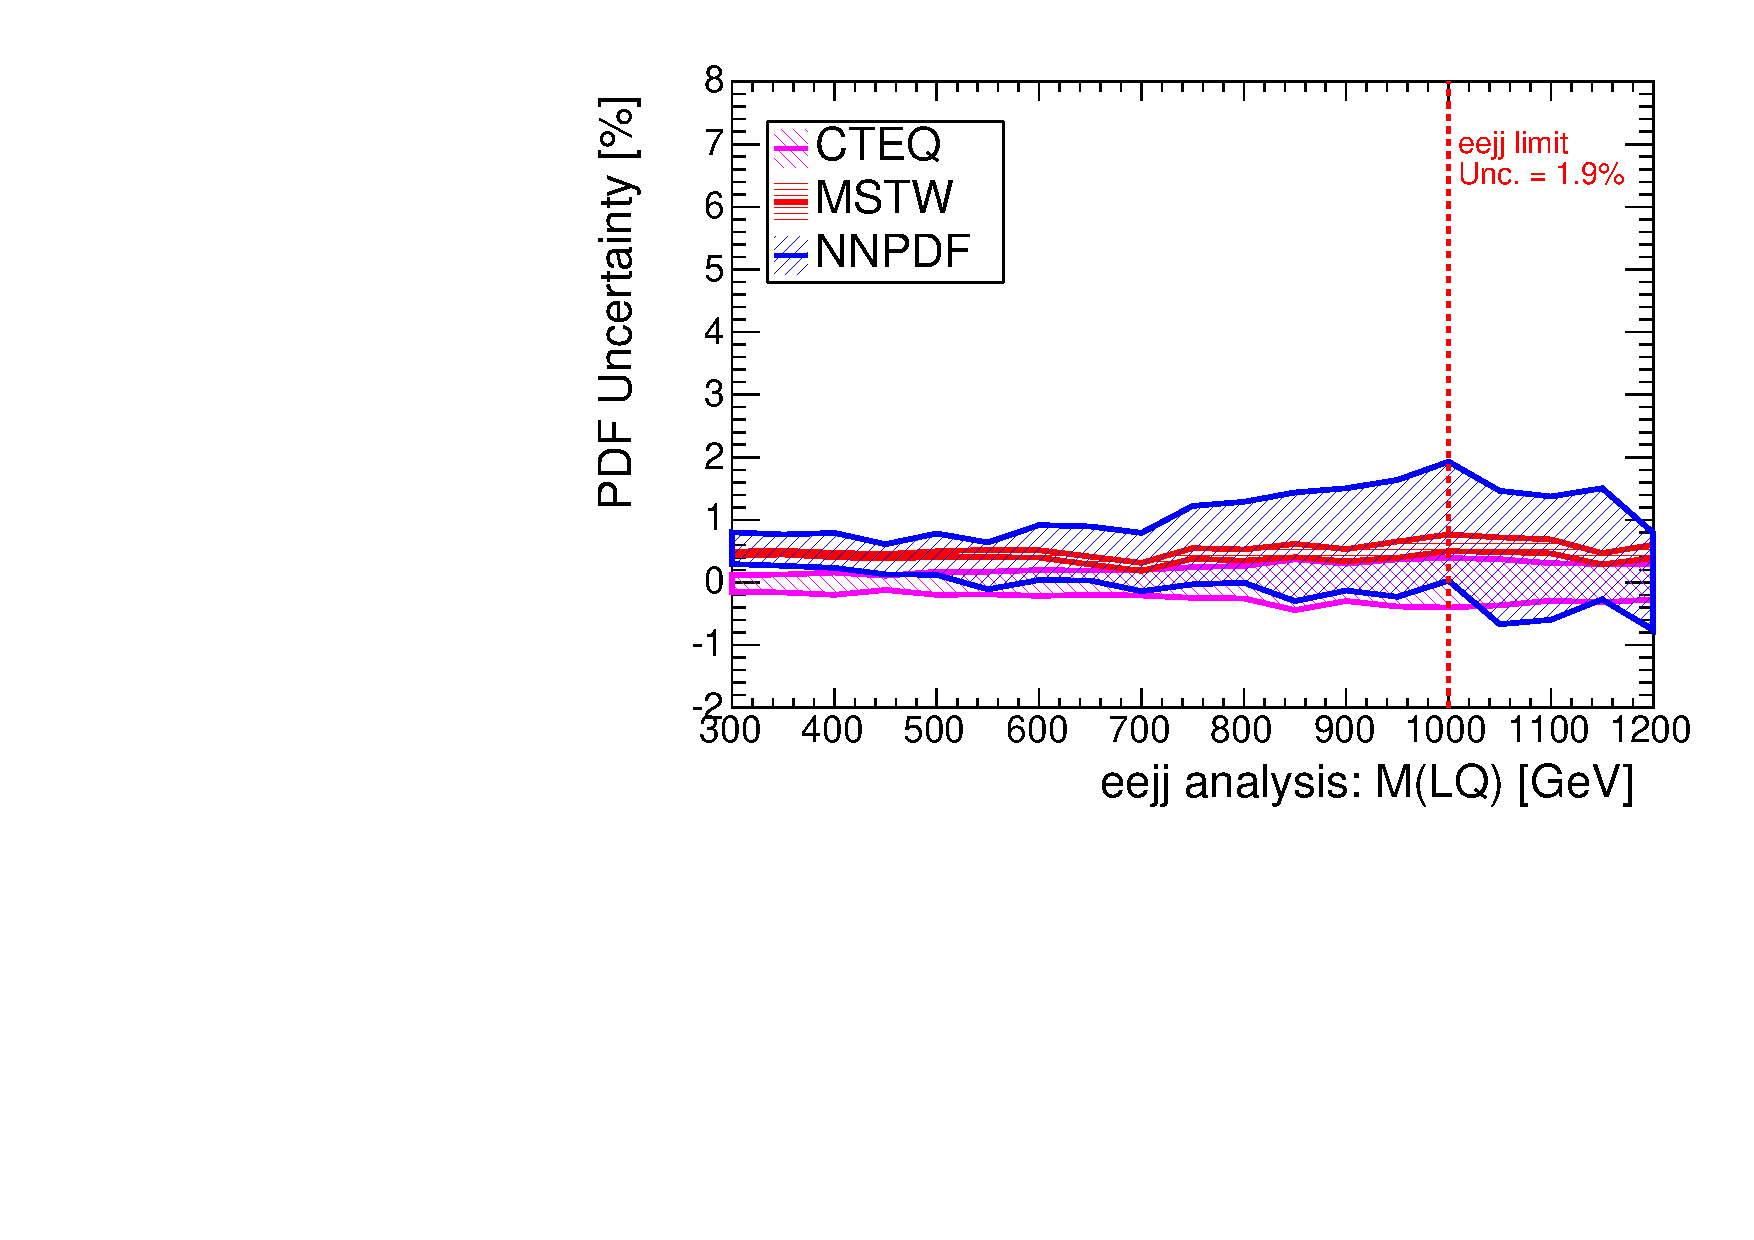
\includegraphics[width=0.6\textwidth]{fig/eejj_envelope.pdf}
%% Text
\label{sec-3-1-1-2}

\centering
\begin{itemize}

\item $x$-axis: LQ mass
\label{sec-3-1-1-2-1}%

\item $y$-axis mean: mean from plots similar to slide 5
\label{sec-3-1-1-2-2}%

\item $y$-axis width: RMS from plots similar to slide 5
\label{sec-3-1-1-2-3}%

\end{itemize} % ends low level
\end{frame}
\begin{frame}
\frametitle{Method for determining final uncertainty}
\label{sec-3-1-2}
\begin{itemize}

\item Quote one uncertainty for all LQ mass selections
\label{sec-3-1-2-1}%

\item If there are no MC events passing a given selection, we can't evaluate PDF uncertainty at that selection level
\label{sec-3-1-2-2}%

\item If there are MC events passing the selection at the LQ limit (1050 GeV for eejj, 850 GeV for evjj):
\label{sec-3-1-2-3}%
\begin{itemize}

\item Use the uncertainty evaluated \alert{at the LQ limit}
\label{sec-3-1-2-3-1}%
\end{itemize} % ends low level

\item Otherwise:
\label{sec-3-1-2-4}%
\begin{itemize}

\item Use the \alert{maximum} evaluated uncertainty
\label{sec-3-1-2-4-1}%
\end{itemize} % ends low level
\end{itemize} % ends low level
\end{frame}
\begin{frame}
\frametitle{PDF uncertainty: eejj background}
\label{sec-3-1-3}
\begin{columns} % Plots
\label{sec-3-1-3-1}
\begin{column}{0.55\textwidth}
%% Plot 1
\label{sec-3-1-3-1-1}

\centering
$\text{Z}+\text{jets}$ MC
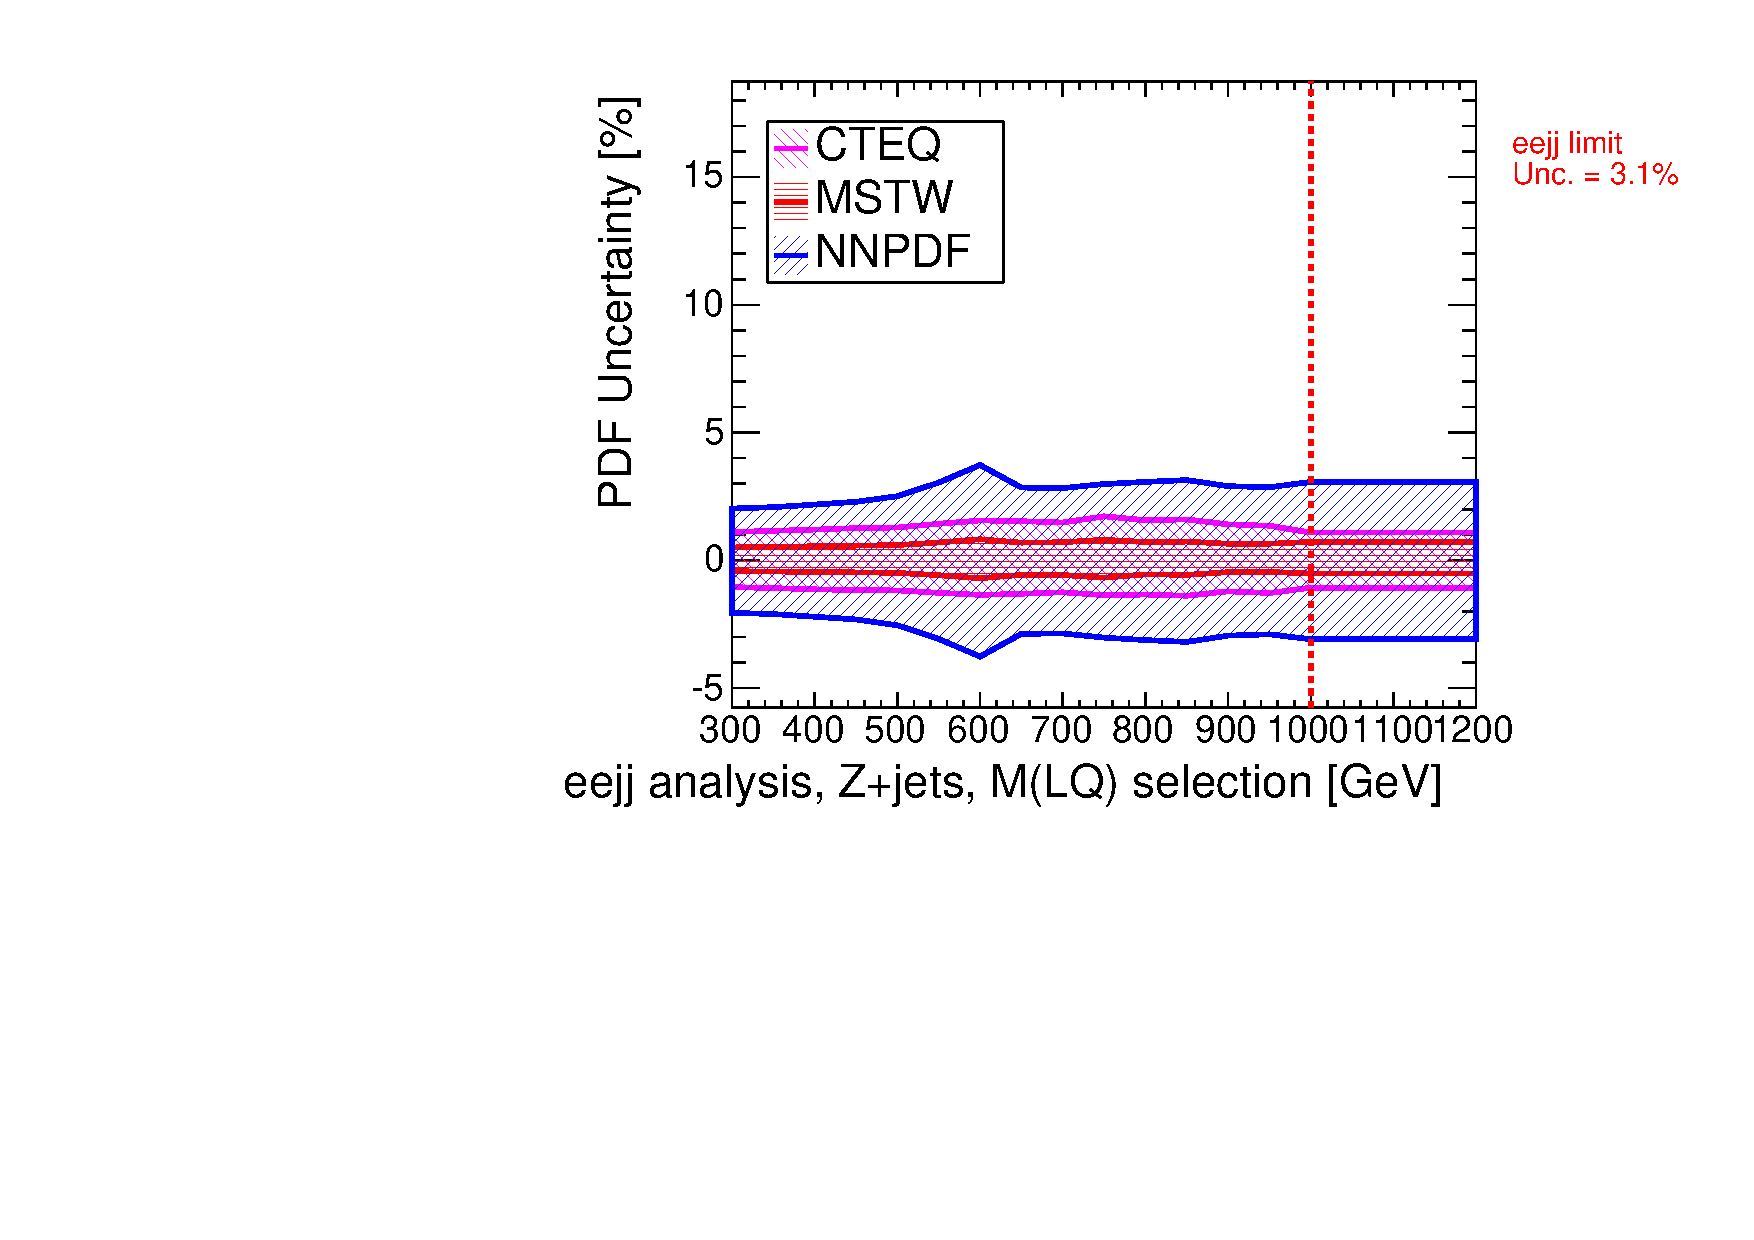
\includegraphics[width=\textwidth]{fig/ZJet_Madgraph_eejj_envelope.pdf}
\end{column}
\begin{column}{0.55\textwidth}
%% Plot 2
\label{sec-3-1-3-1-2}

\centering
$t\bar{t}$ MC (not used)
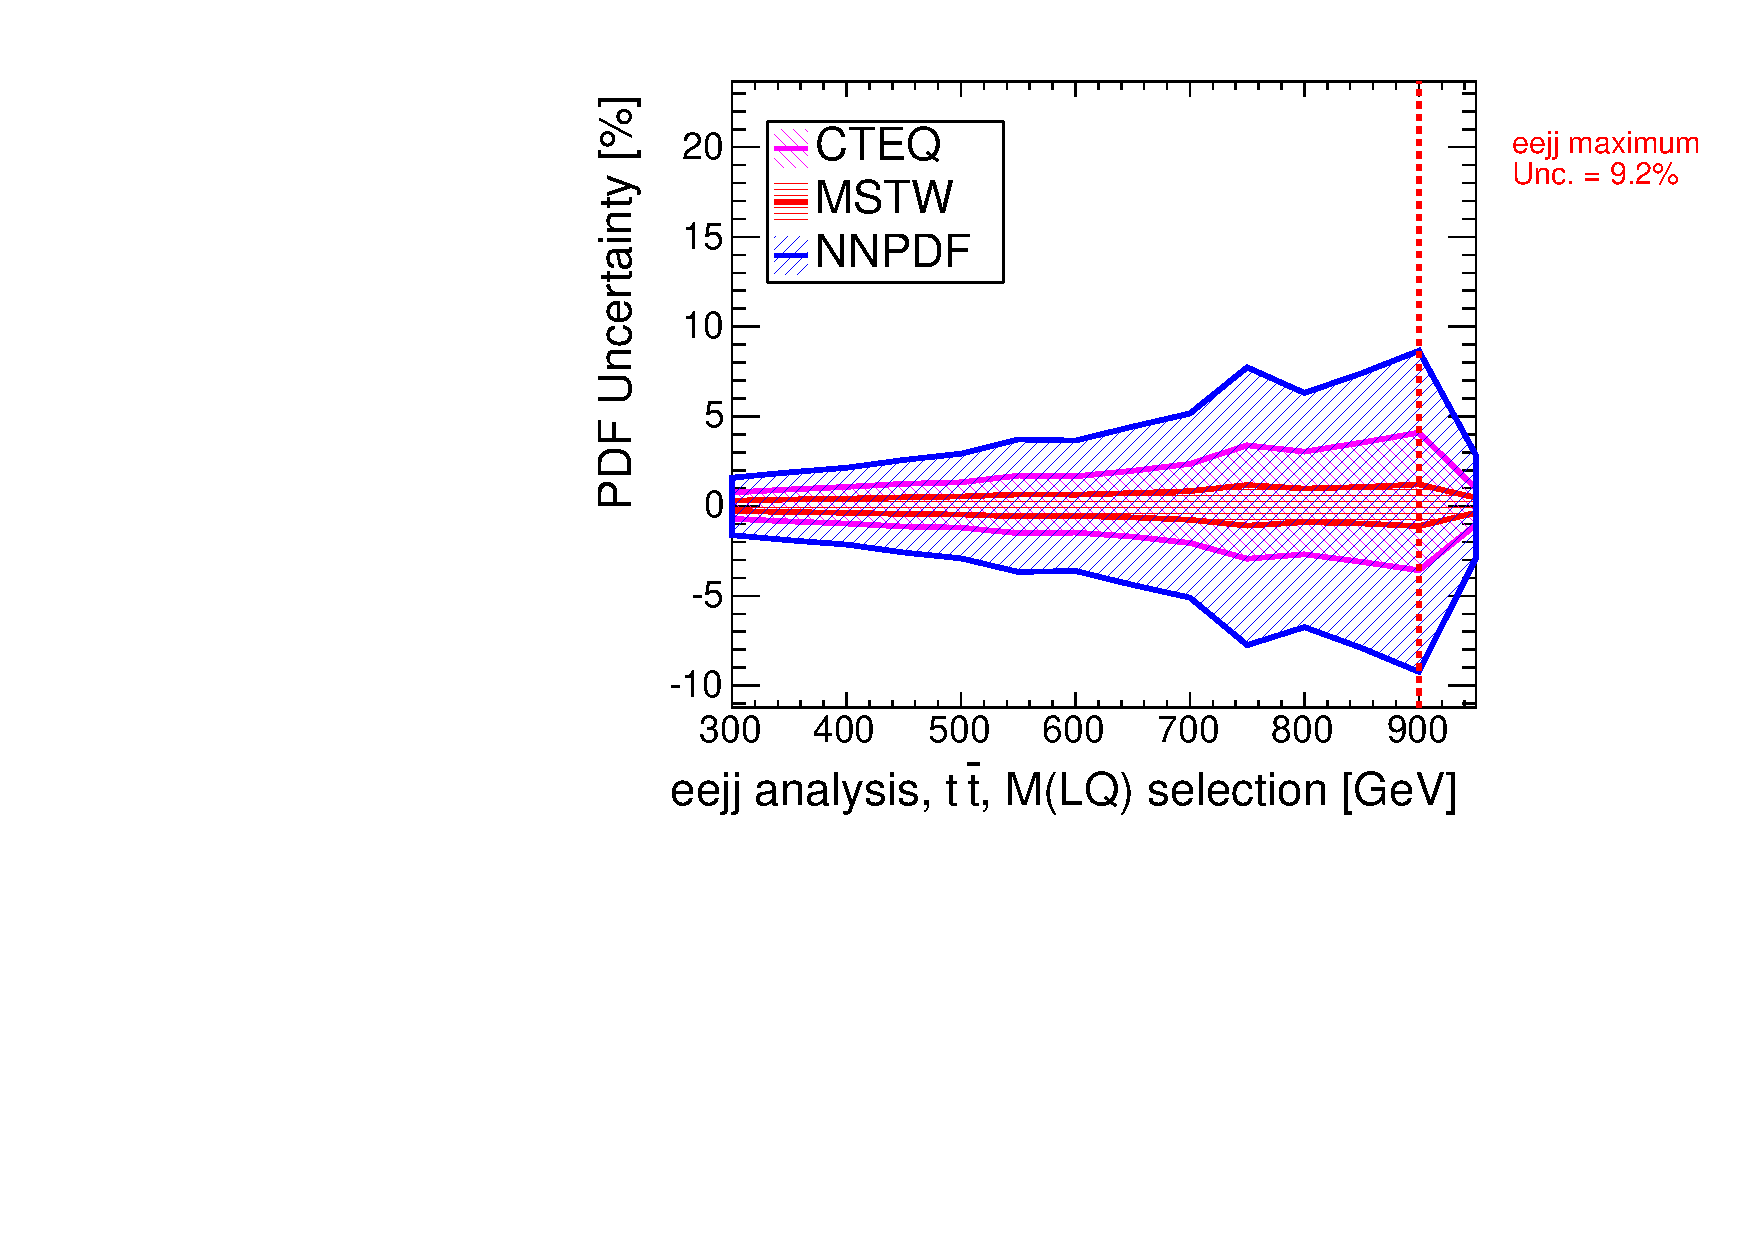
\includegraphics[width=\textwidth]{fig/TTbar_Madgraph_eejj_envelope.pdf}
\end{column}
\end{columns}
%% Text
\label{sec-3-1-3-2}

\centering
\begin{itemize}

\item $x$-axis: LQ mass
\label{sec-3-1-3-2-1}%

\item $y$-axis mean: mean from plots similar to slide 5
\label{sec-3-1-3-2-2}%

\item $y$-axis width: RMS from plots similar to slide 5
\label{sec-3-1-3-2-3}%

\end{itemize} % ends low level
\end{frame}
\begin{frame}
\frametitle{PDF uncertainty: evjj signal}
\label{sec-3-1-4}
%% Plot
\label{sec-3-1-4-1}

\centering
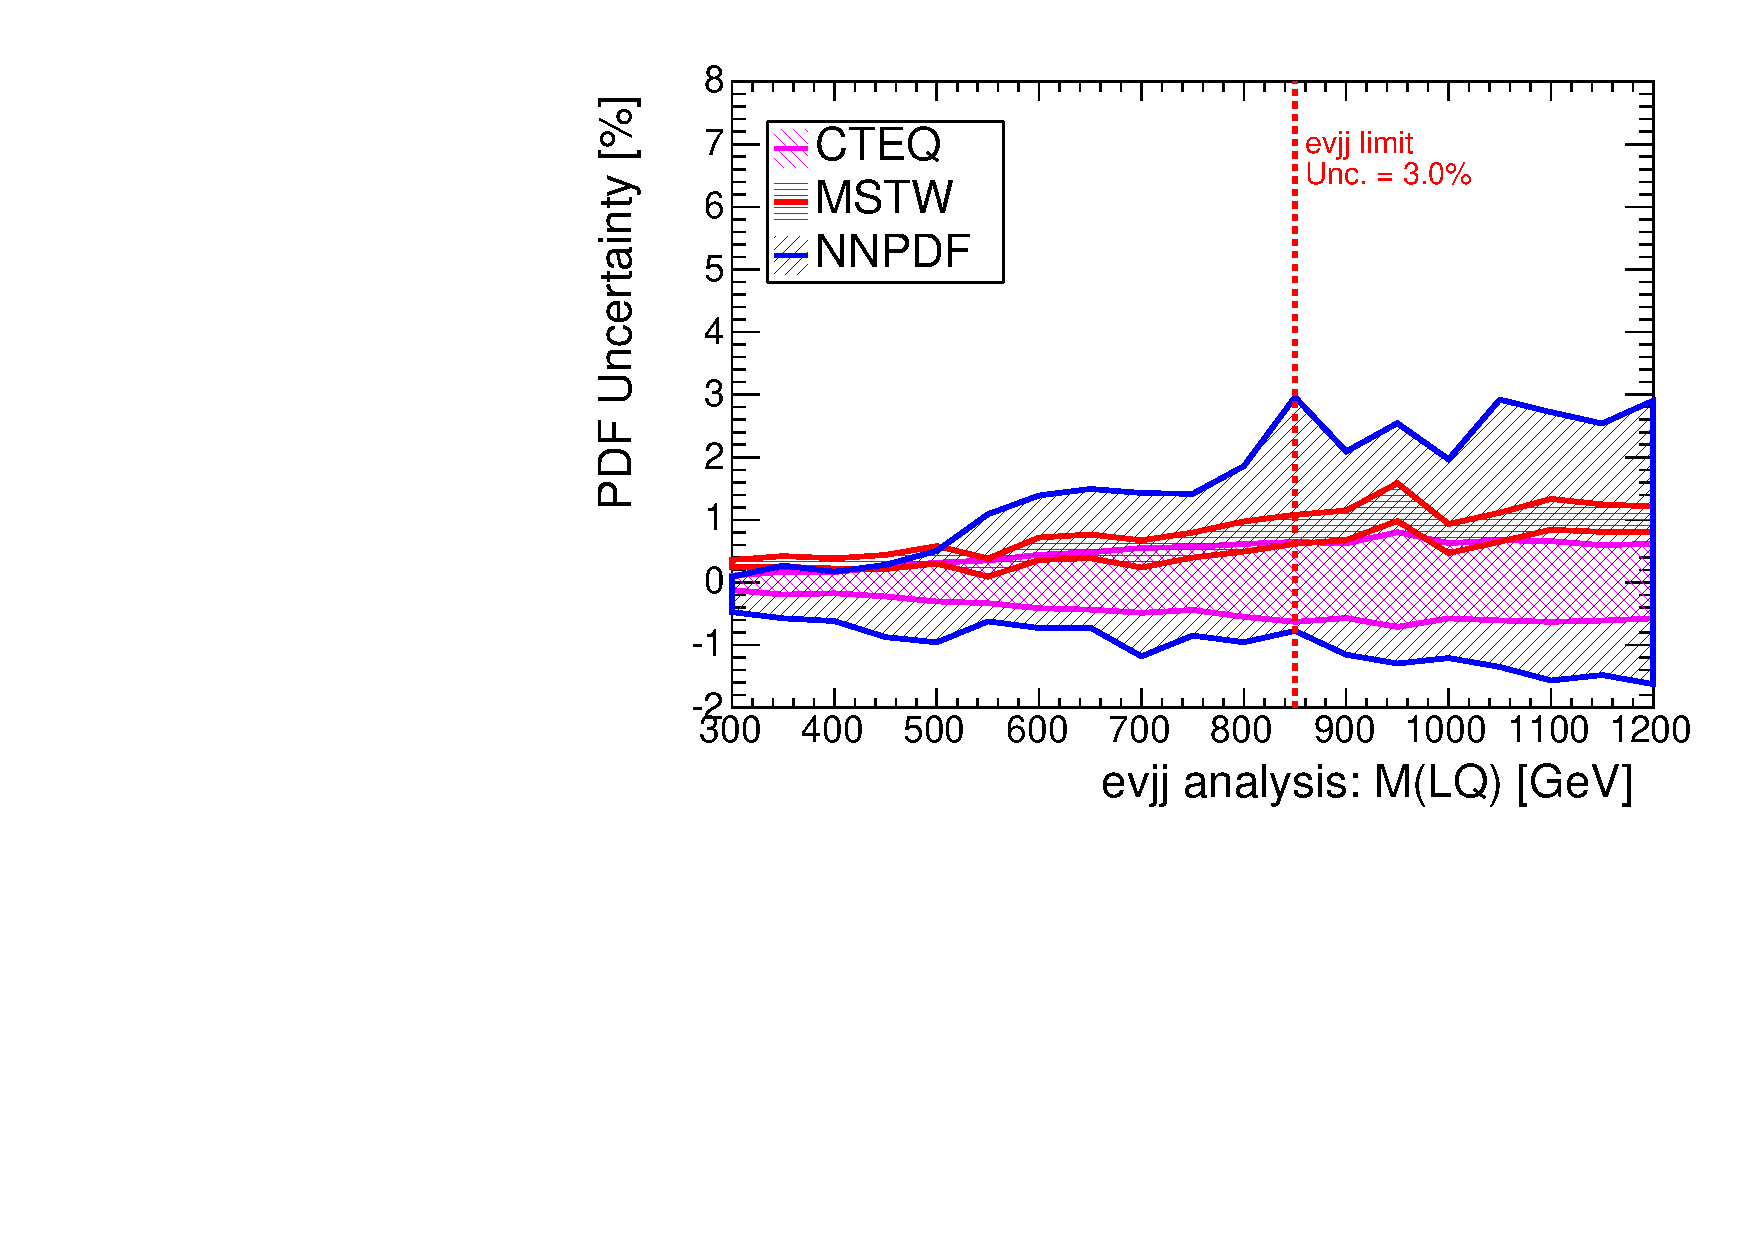
\includegraphics[width=0.6\textwidth]{fig/enujj_envelope.pdf}
%% Text
\label{sec-3-1-4-2}

\centering
\begin{itemize}

\item $x$-axis: LQ mass
\label{sec-3-1-4-2-1}%

\item $y$-axis mean: mean from plots similar to slide 5
\label{sec-3-1-4-2-2}%

\item $y$-axis width: RMS from plots similar to slide 5
\label{sec-3-1-4-2-3}%
\end{itemize} % ends low level
\end{frame}
\begin{frame}
\frametitle{PDF uncertainty: evjj background}
\label{sec-3-1-5}
\begin{columns} % Plots
\label{sec-3-1-5-1}
\begin{column}{0.55\textwidth}
%% Plot 1
\label{sec-3-1-5-1-1}

\centering
$\text{W}+\text{jets}$ MC
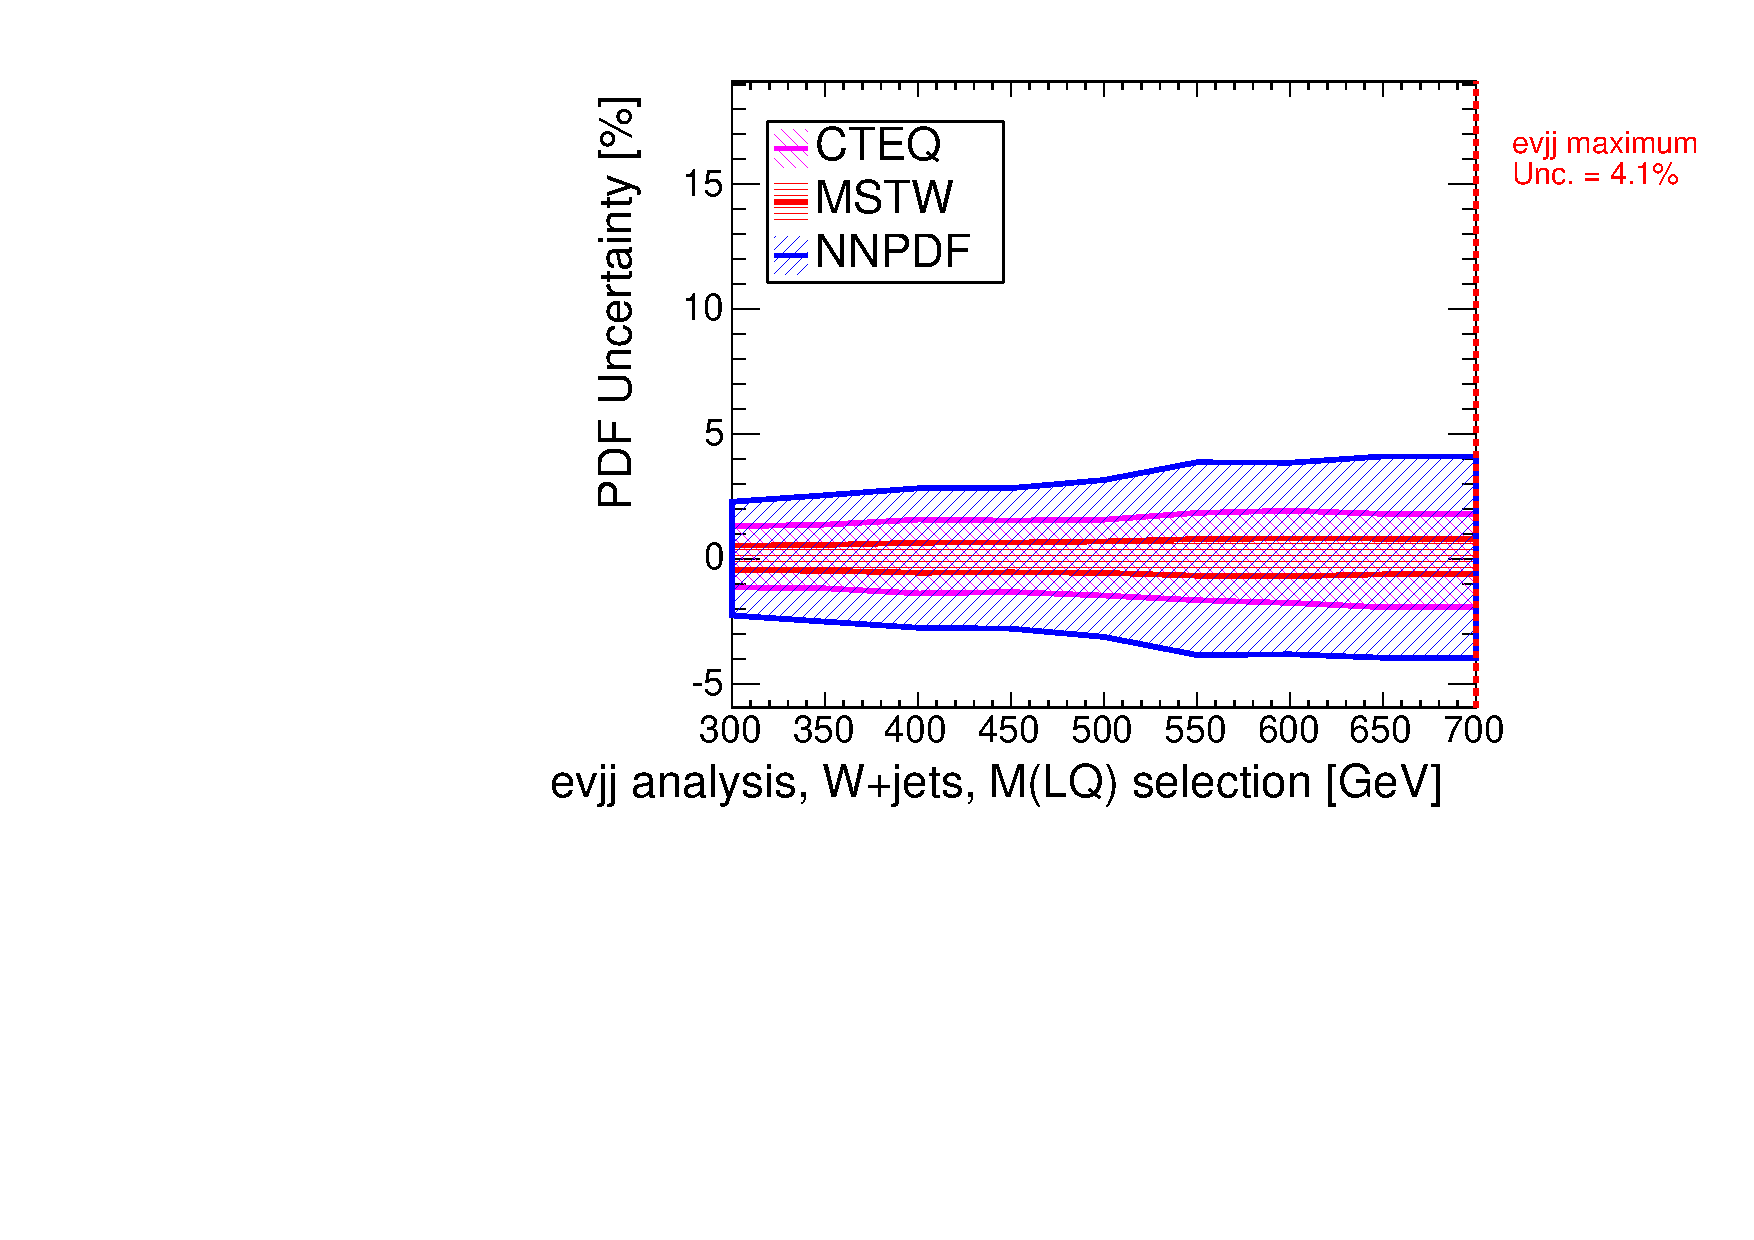
\includegraphics[width=\textwidth]{fig/WJet_Madgraph_enujj_envelope.pdf}
\end{column}
\begin{column}{0.55\textwidth}
%% Plot 2
\label{sec-3-1-5-1-2}

\centering
$t\bar{t}$ MC
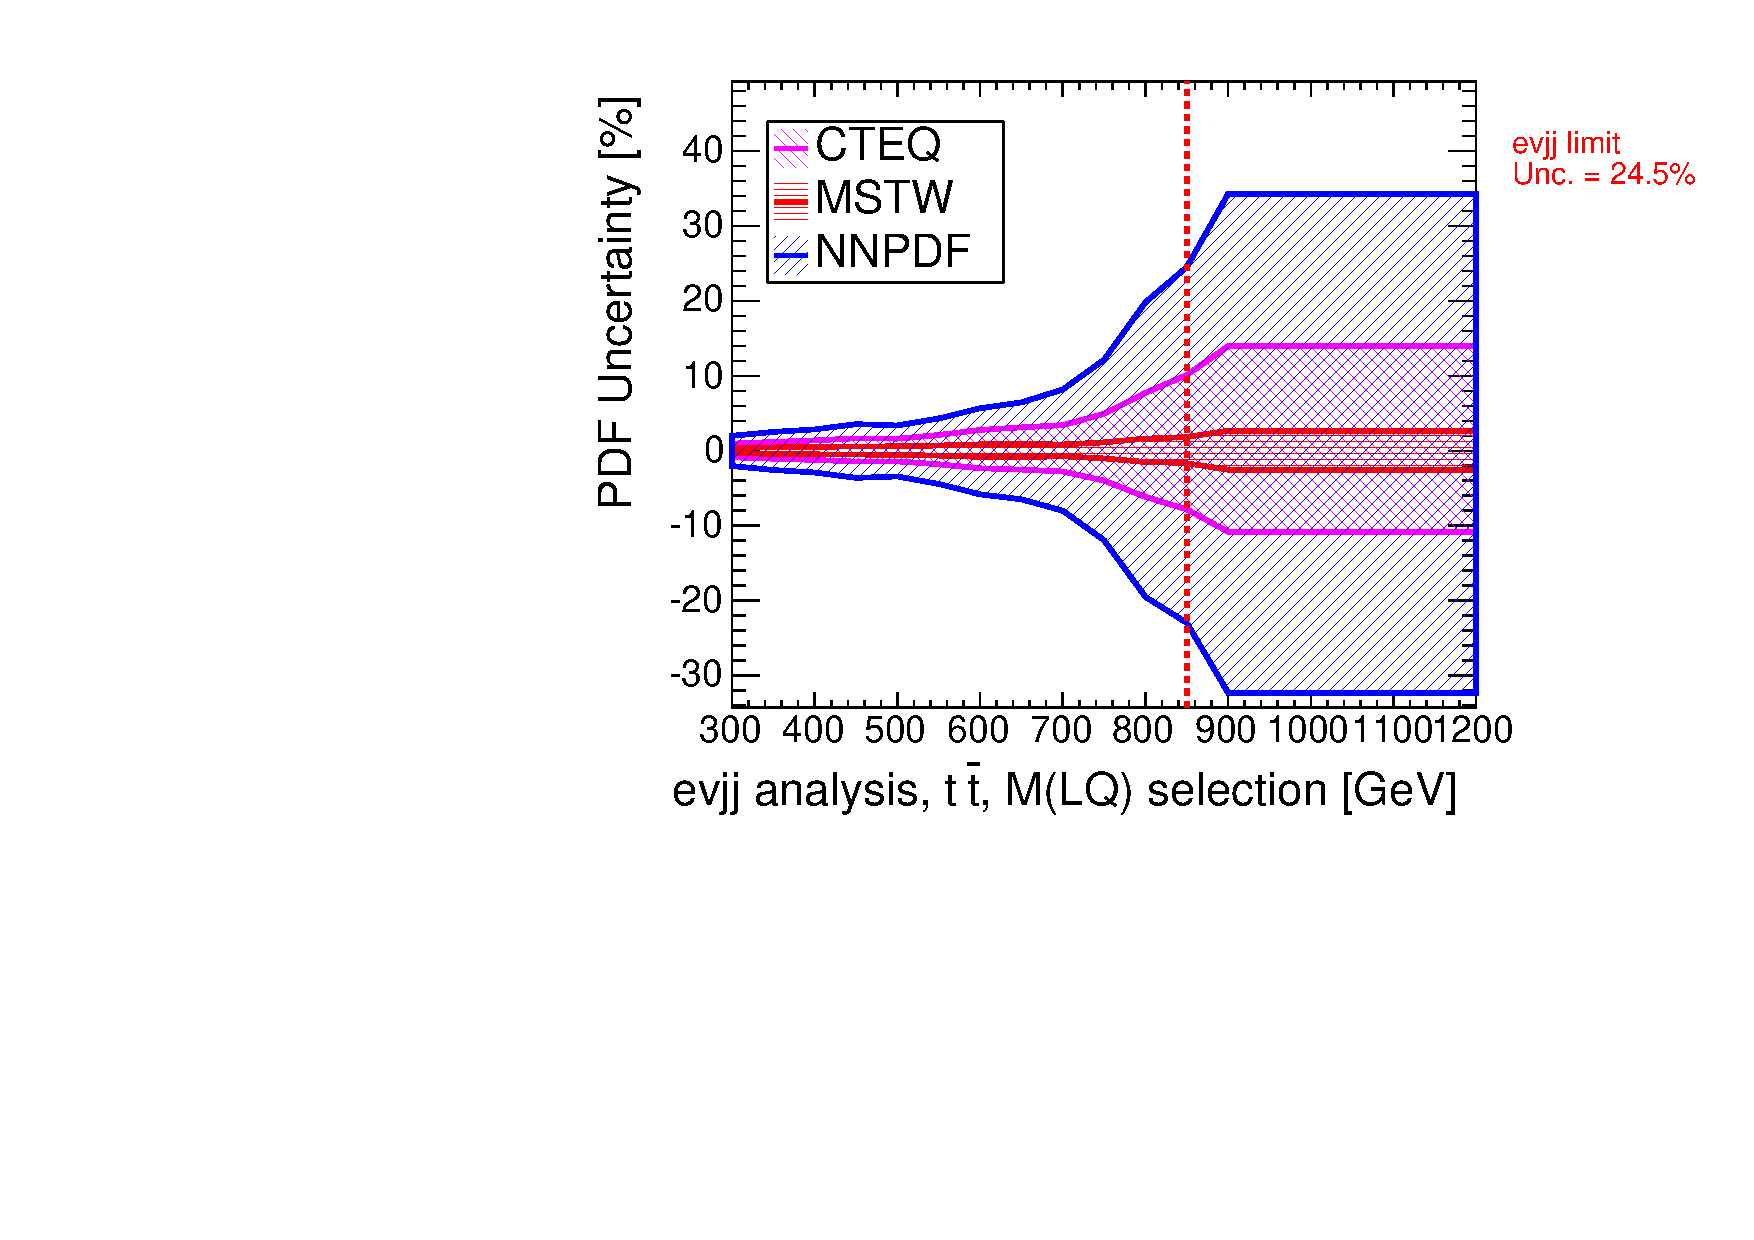
\includegraphics[width=\textwidth]{fig/TTbar_Madgraph_enujj_envelope.pdf}
\end{column}
\end{columns}
%% Text
\label{sec-3-1-5-2}

\centering
\begin{itemize}

\item $x$-axis: LQ mass
\label{sec-3-1-5-2-1}%

\item $y$-axis mean: mean from plots similar to slide 5
\label{sec-3-1-5-2-2}%

\item $y$-axis width: RMS from plots similar to slide 5
\label{sec-3-1-5-2-3}%

\end{itemize} % ends low level
\end{frame}
\section{Conclusion}
\label{sec-4}
\subsection{Conclusion}
\label{sec-4-1}
\begin{frame}
\frametitle{Conclusion}
\label{sec-4-1-1}
\begin{itemize}

\item Signal PDF uncertainties:
\label{sec-4-1-1-1}%
\begin{itemize}

\item eejj: 2\%
\label{sec-4-1-1-1-1}%

\item evjj: 3\%
\label{sec-4-1-1-1-2}%
\end{itemize} % ends low level

\item Background PDF uncertainties:
\label{sec-4-1-1-2}%
\begin{itemize}

\item eejj $\text{Z}+\text{jets}$: 3\%
\label{sec-4-1-1-2-1}%

\item evjj $\text{W}+\text{jets}$: 4\%
\label{sec-4-1-1-2-2}%

\item evjj $t\bar{t}$: \alert{25\%}
\label{sec-4-1-1-2-3}%
\end{itemize} % ends low level

\item Why is the evjj $t\bar{t}$ uncertainty so high?  Possible answer:
\label{sec-4-1-1-3}%
\begin{itemize}

\item Final acceptance is \alert{very} low (but not zero) for $t\bar{t}$ MC
\label{sec-4-1-1-3-1}%

\item Only 8 events pass M(LQ) = 850 selection (evjj limit)
\label{sec-4-1-1-3-2}%

\item Extremely hard cuts imply larger PDF uncertainties
\label{sec-4-1-1-3-3}%
\end{itemize} % ends low level
\end{itemize} % ends low level
\end{frame}

\end{document}
